\documentclass[tikz,border=3pt]{standalone}
\usepackage{libertine}
\usetikzlibrary{arrows.meta,positioning,calc,fit,backgrounds}
\definecolor{navy}{HTML}{183A61}
\definecolor{blue}{HTML}{377EB8}
\definecolor{bluefill}{HTML}{EAF3FB}
\definecolor{orange}{HTML}{D07820}
\definecolor{orangefill}{HTML}{FFF3E5}
\definecolor{green}{HTML}{4F8A68}
\definecolor{greenfill}{HTML}{EEF8F1}
\definecolor{slate}{HTML}{66778B}
\definecolor{grayfill}{HTML}{F5F7FA}
\tikzset{
  module/.style={rounded corners=2pt, draw=blue, fill=bluefill, line width=.75pt,
    minimum height=8mm, text width=3.1cm, align=center, font=\scriptsize\bfseries, text=navy},
  ctlmodule/.style={module, draw=orange, fill=orangefill, text=orange},
  realmodule/.style={module, draw=green, fill=greenfill, text=green},
  memory/.style={module, draw=slate, fill=grayfill},
  region/.style={rounded corners=4pt, draw=slate, fill=white, line width=.8pt},
  fpga/.style={region, draw=blue}, host/.style={region, draw=orange, fill=orangefill!30},
  backend/.style={region, draw=green, fill=greenfill!28},
  ctrl/.style={-{Stealth[length=2.1mm]}, draw=orange, line width=.95pt},
  ctrlbi/.style={{Stealth[length=2.1mm]}-{Stealth[length=2.1mm]}, draw=orange, line width=.95pt},
  data/.style={{Stealth[length=2.2mm]}-{Stealth[length=2.2mm]}, draw=blue, line width=1.3pt},
  elabel/.style={font=\tiny, fill=white, inner sep=1pt, text=slate}
}
\begin{document}
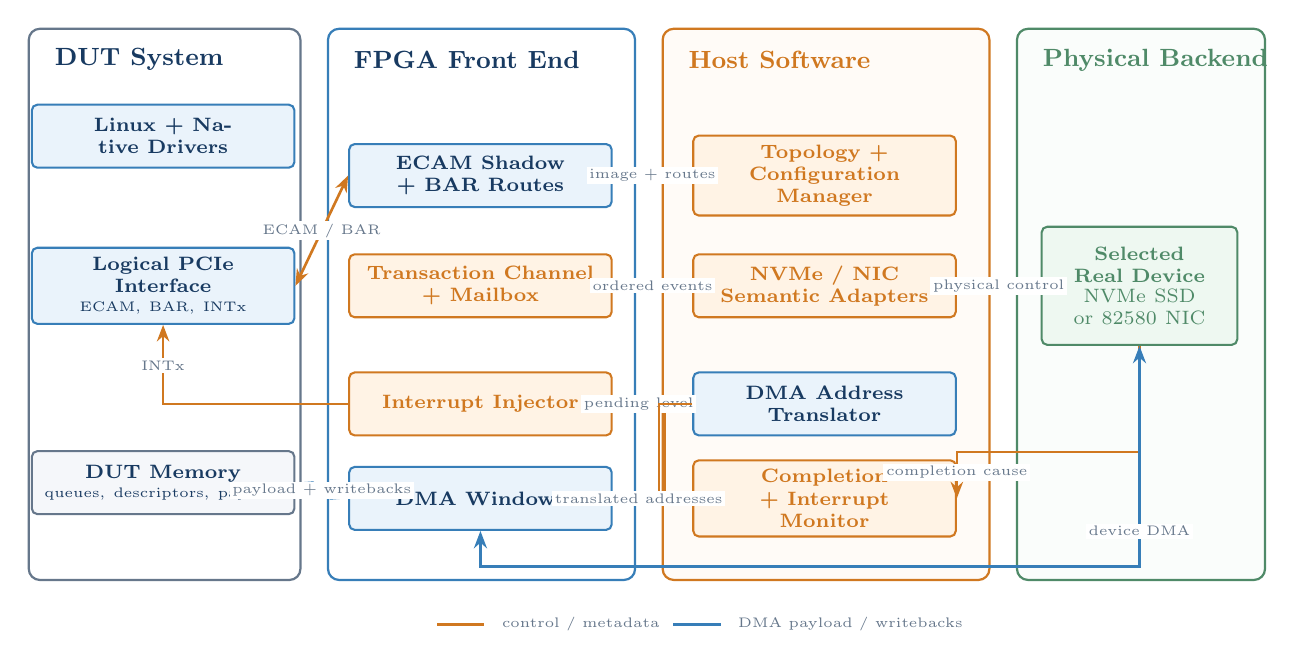
\begin{tikzpicture}[x=1cm,y=1cm]
  \begin{scope}[on background layer]
    \node[region, minimum width=3.45cm, minimum height=7.0cm, anchor=south west] at (0,0) {};
    \node[fpga, minimum width=3.9cm, minimum height=7.0cm, anchor=south west] at (3.8,0) {};
    \node[host, minimum width=4.15cm, minimum height=7.0cm, anchor=south west] at (8.05,0) {};
    \node[backend, minimum width=3.15cm, minimum height=7.0cm, anchor=south west] at (12.55,0) {};
  \end{scope}
  \node[anchor=west, font=\small\bfseries, text=navy] at (.22,6.62) {DUT System};
  \node[anchor=west, font=\small\bfseries, text=navy] at (4.02,6.62) {FPGA Front End};
  \node[anchor=west, font=\small\bfseries, text=orange] at (8.27,6.62) {Host Software};
  \node[anchor=west, font=\small\bfseries, text=green] at (12.77,6.62) {Physical Backend};

  \node[module] (driver) at (1.72,5.65) {Linux + Native Drivers};
  \node[module] (root) at (1.72,3.75) {Logical PCIe Interface\\[-1pt]\normalfont\tiny ECAM, BAR, INTx};
  \node[memory] (mem) at (1.72,1.25) {DUT Memory\\[-1pt]\normalfont\tiny queues, descriptors, payload};

  \node[module] (ecam) at (5.75,5.15) {ECAM Shadow + BAR Routes};
  \node[ctlmodule] (event) at (5.75,3.75) {Transaction Channel\\+ Mailbox};
  \node[ctlmodule] (irq) at (5.75,2.25) {Interrupt Injector};
  \node[module] (dma) at (5.75,1.05) {DMA Windows};

  \node[ctlmodule] (topo) at (10.12,5.15) {Topology + Configuration\\Manager};
  \node[ctlmodule] (adapter) at (10.12,3.75) {NVMe / NIC\\Semantic Adapters};
  \node[module] (xlat) at (10.12,2.25) {DMA Address Translator};
  \node[ctlmodule] (monitor) at (10.12,1.05) {Completion + Interrupt\\Monitor};

  \node[realmodule, text width=2.25cm, minimum height=15mm] (device) at (14.12,3.75)
    {Selected Real Device\\[-1pt]\normalfont\scriptsize NVMe SSD or 82580 NIC};

  \draw[ctrlbi] (root.east) -- node[elabel] {ECAM / BAR} (ecam.west);
  \draw[ctrl] (topo.west) -- node[elabel] {image + routes} (ecam.east);
  \draw[ctrlbi] (event.east) -- node[elabel] {ordered events} (adapter.west);
  \draw[ctrl] (adapter.east) -- node[elabel] {physical control} (device.west);
  \draw[ctrl] (device.south) -- ++(0,-1.35) -| node[elabel, pos=.72] {completion cause} (monitor.east);
  \draw[ctrl] (monitor.west) -- ++(-.35,0) |- node[elabel, pos=.75] {pending level} (irq.east);
  \draw[ctrl] (irq.west) -- ++(-.48,0) -| node[elabel, pos=.74] {INTx} (root.south);
  \draw[ctrl] (xlat.west) -- ++(-.42,0) |- node[elabel, pos=.72] {translated addresses} (dma.east);
  \draw[data] (mem.east) -- node[elabel] {payload + writebacks} (dma.west);
  \draw[data] (dma.south) -- ++(0,-.45) -| node[elabel, pos=.58] {device DMA} (device.south);

  \draw[orange, line width=1.05pt] (5.2,-.55) -- (5.8,-.55);
  \node[anchor=west, font=\tiny, text=slate] at (5.9,-.55) {control / metadata};
  \draw[blue, line width=1.35pt] (8.2,-.55) -- (8.8,-.55);
  \node[anchor=west, font=\tiny, text=slate] at (8.9,-.55) {DMA payload / writebacks};
\end{tikzpicture}
\end{document}
